% \documentclass{IEEEtran}
\documentclass[12pt]{article}
\usepackage[utf8]{inputenc}

\usepackage[margin=1in]{geometry}

\usepackage{librebaskerville}
\usepackage[T1]{fontenc}

\usepackage{setspace}
\doublespacing

\usepackage{url}
\def\UrlBreaks{\do\/\do-}

\usepackage{graphicx}
\usepackage[labelformat=empty]{caption}
\usepackage{subcaption}
\usepackage{notoccite}

% \usepackage{xcolor}
% \pagecolor[rgb]{0.1,0.1,0.1}
% \color[rgb]{0.7,0.7,0.7}

\newenvironment{quote_1in}%
  {\list{}{\leftmargin=1in\rightmargin=1in}\item[]}%
  {\endlist}

\interfootnotelinepenalty=10000

\setlength{\parskip}{\baselineskip}
\setlength{\parindent}{0pt}

\widowpenalty10000
\clubpenalty10000

\title{Automated Authority \\[-6pt]
%    \bigskip \large \textit{or \\ How I Learned to Give Up Control and Love our Robot Overlords \vspace{-\baselineskip}}
}
\author{\vspace{-\baselineskip}Peter Lillian}
\date{\vspace{-\baselineskip}July 2019}

\begin{document}

\frenchspacing

\maketitle


% \begin{quote}
%     "When the Gaon saw that the Golem was growing larger and larger, he feared that the Golem would destroy the universe. He then removed the Holy Name that was embedded on his forehead, thus causing him to disintegrate and return to dust." \cite{altona}
% \end{quote}

\begin{quote_1in}
    \textit{When Marduk commanded me to give justice to the people of the land and to let them have good governance, I set forth... to make justice appear in the land, to destroy the evil and the wicked, that the strong might not oppress the weak.}
    
    ---Hammurabi of Babylonia \cite{driver2007babylonian}
\end{quote_1in}

All governments throughout history have been run by humans. Some have claimed to serve the people of their society---others have blatantly served a different goal.
% The first ever governments arose in the ancient Levant: the so-called cradle of civilization. The first cities were formed here by necessity. Warring tribes recently taken to agriculture needed to allocate resources and plan for the future \cite{maisels2003emergence}. As time went on and the empires became larger, governments became more complex.
In the modern era, and governments play a larger role in human life than ever before---everything from education to urban planning is a function of the state. But have the motivations of governments improved? The Bulletin of Atomic Scientists considers the current political climate "as worrisome as the most dangerous times of the Cold War" \cite{mecklin2019new}.
\begin{figure}[ht]
\centering
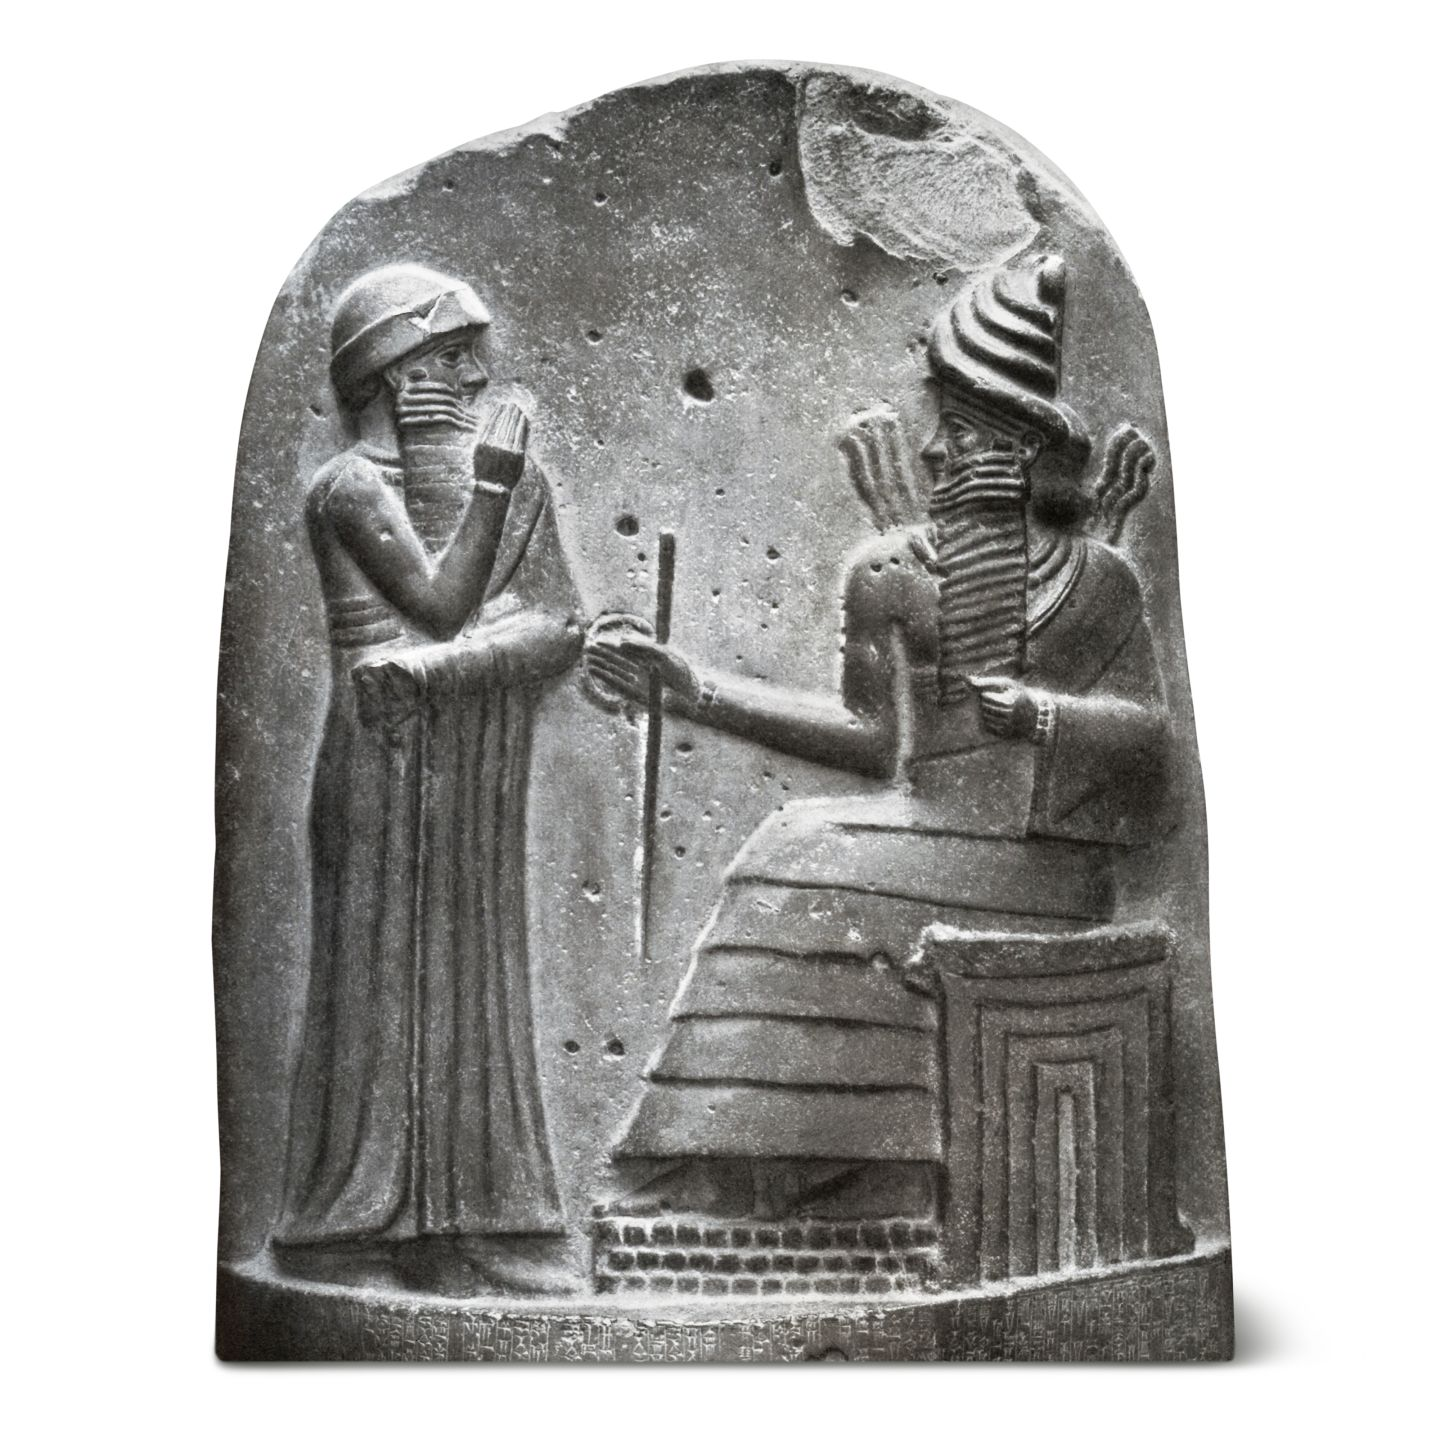
\includegraphics[width=0.75\textwidth]{babylon.jpg}
\begin{quote_1in}
    \caption{
    \textit{Marduk, ruler of the gods, gives legal power to Hammurabi, king of Babylonia} \cite{babylon}}
\end{quote_1in}
\end{figure}
Climate change has gotten to the point where many experts consider it unavoidable \cite{ghosh2018great}. Wealth inequality throughout the developed world has been getting worse \cite{knight2017wealth}. % We can see this in some of the worst decisions in history: Napoleon's invasion of Russia, China's Cultural Revolution, or New Coke.
Humans tend to be self-serving, fail to think long-term, and exhibit bias towards members of their own groups, among many other pitfalls \cite{haselton2006paranoid}.
% These flaws are compounded in organizations around the world, as all institutions are made up of humans---and the whole is a sum of its parts.
It is this kind of flawed decision-making, typical of \textit{Homo sapiens}, that causes so much calamity.

With these flaws, we won't be ruling the Earth forever. Artificial Intelligence is improving by the day. According to the International Data Corporation, global spending on AI is expected to double by 2022 to almost \$80 billion \cite{globalAI}. In the wake of this windfall, we'll start to see more intelligent systems---machines eventually capable of performing all tasks better than humans \cite{bostrom2005history}. What then? The stakeholders in the future of AI include not only the human race, but also life on Earth and potentially the entire universe---we can use the utility ethics test to examine these scenarios. Should we put limits on AI to keep humans employed? A Luddite approach will only hold us back, as governments or corporations that implement these kind of regulations will inevitably be outcompeted by those that do not. Even if the whole world got together and agreed to put anti-AI laws into place (good luck getting North Korea or the Mafia to agree to that anyway), what would be the purpose of making humans do jobs robots can do better? Do we still have people draw spreadsheets by hand?
\begin{figure}[b!]
\bigskip
\centering
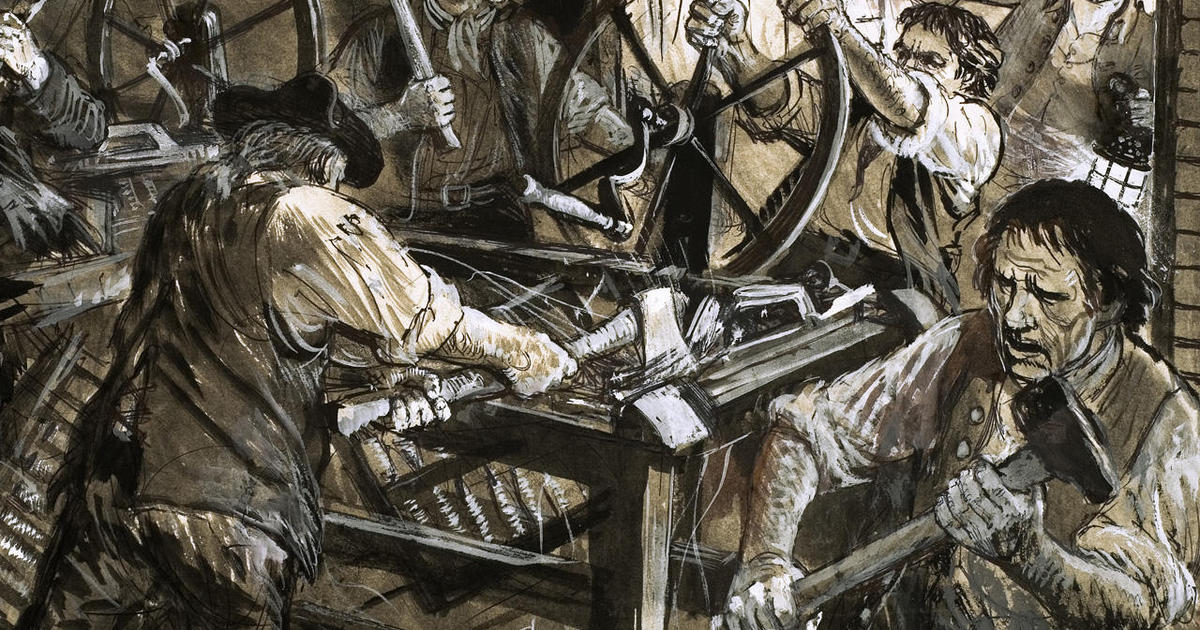
\includegraphics[width=0.75\textwidth]{luddites.jpg}
\begin{quote_1in}
    \caption{
    \textit{Luddites, a group of textile workers, destroy the textile mills that replaced their jobs.} \cite{luddites}}
\end{quote_1in}
\end{figure}
Of course, Microsoft Excel isn't going to revolt against us anytime soon, but for the purposes of this paper we will assume that we have solved the superintelligent control problem (as this is a technical challenge) and are able to create friendly AI that won't harm us.\footnote{A discussion of the dangers of unfriendly AI is out of scope here, but the curious reader will find Nick Bostrom's \textit{Superintelligence: Paths, Dangers, Strategies} \cite{bostrom2014superintelligence} to be an enlightening overview of the topic.}
There is one job, though, that might seem smart to keep as a human occupation. Leadership---an especially valued human quality---will likely be the last job handed over to the machines. For our own sakes, it shouldn't be.
Though it may scare some people, putting AI into power will make a smarter, faster, and more equitable world. % thesis

% It would seem rational to give power to an agent that is intelligent, but the smartest aren't always in office: just look at our current leaders. It would seem shrewd to give power to an agent that can respond fast to threats, but how will people feel about a nonhuman intelligence? It would seem smart to give power to an agent programmed to act in the interest of the people, but how could they trust it?

In order to examine these questions, we can look at an automated authority from the perspective of the utility test. With a machine government, the average person would benefit financially from an improved economy---the AI's superior financial policy would make recessions much less likely and put more money in the pockets of everyday people \cite{ernst2018economics}. In this society, as no humans work, the machines will remove all social classes. With no humans working, it will be impossible to maintain that some humans deserve more wealth. However, this would anger the rich, as their institutions and old-boy networks within the financial system would no longer give them power. In the long-term, though, the incredible abundance produced by a post-scarcity economy (one where robots create endless wealth distributed equally among all humans) might allow everyone the type of luxuriant lifestyle previously only afforded to the few \cite{korinek2017artificial}.

We could also release the source code of this AI so that any interested citizen could literally read the mind of their leader, and even vote on tweaks or improvements. This AI could be programmed to always act in the perfect interest of the people \cite{bostrom2014superintelligence}. If this AI's programming was made open-source, the average person would have much more confidence in their government, something that is sorely lacking in many human regimes today. Of course, while an AI government is great for the citizens, it would be a nightmare for politicians as they would be out of a job---though this might not be all bad, as the European Center for the Governance of Change found that already 1/4 of citizens would prefer AI to their current politicians \cite{euro2019tech}.

A true superintelligence could respond to threats instantly \cite{bostrom2014superintelligence}. An economic crash or surprise war would take human leaders off-guard, but an AI would be able to watch the situation unfold at millions of frames per second. The downside to this, though, is that the public won't be able to react to its decisions in time to modify it. We could create robust guaranteed-friendly AI (that won't kill us), but many members of the public would still hold reservations about this situation, and this could make them more unhappy under the new government. Yet after generations of successful machine rule, it is unlikely that people would continue to harbor these views.

One task humans are notoriously bad at is long-term planning \cite{dorner1994errors}, a kind of thinking that is a natural strength of machines \cite{bostrom2003ethical}. Avoidable catastrophes like climate change, which our governments have utterly failed to address \cite{ghosh2018great}, would not happen to civilizations run by AI, as they would be built with real long-term planning abilities. This means that the Earth and the environment would greatly benefit from governments actually understanding how risky actions like logging the Amazon can be. With this kind of planning, governments will be able to address existential risks\footnote{Existential risks are risks to the continued survival of life on this planet or in the universe \cite{bostrom2011global}.} like asteroid impacts or global pandemics \cite{bostrom2011global}. An AI government would also be adept at finding and dealing with threats we can't forsee, such as dangers from other disruptive technologies (e.g. nanotech) or gamma ray bursts, any of which could easily wipe out life on earth \cite{bostrom2011global}.

\begin{figure}[t!]
\bigskip
\centering
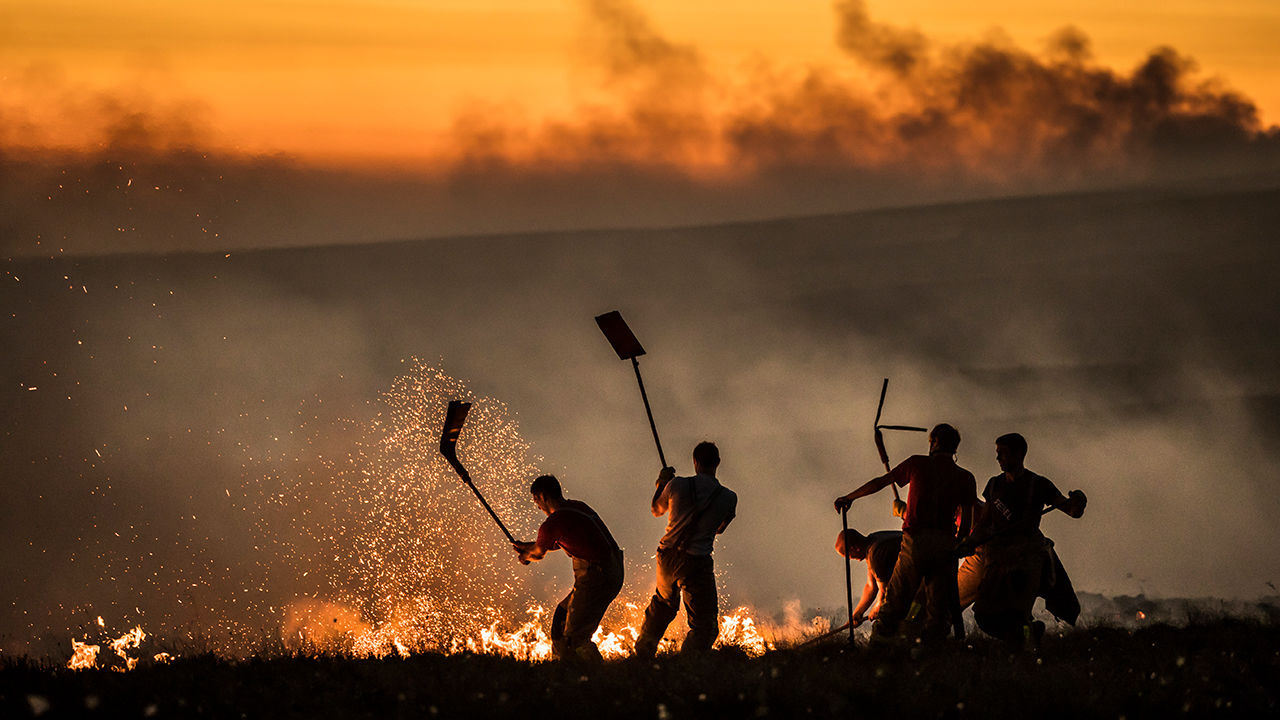
\includegraphics[width=0.75\textwidth]{fire.jpg}
\begin{quote_1in}
    \caption{
    \textit{Firefighters tackle a blaze near Boston, MA. Humans tend to solve the short-term problem (fight the fire) but not the long-term problem (end climate change).} \cite{fire}}
\end{quote_1in}
\end{figure}

If we decided not to implement an AI government, a very different set of outcomes emerges. The biggest immediate issue? AI use spreads to almost all industries; businesses realize to stay competitive they need to replace their CEOs with machines \cite{bostrom2014superintelligence}. This means that suddenly we have a government, which is tasked with the regulation and control of private industry, trying to keep up with AI that evolve by the hour. Think about how tech-illiterate our current politicians are, unable to ask relevant questions at Facebook hearings \cite{rampell2018internet}. Imagine them trying to control organizations run by AI at the speed of thought. They'd be outclassed like a monkey trying to run the circus.

With government oversight of the economy made impossible, the ultra-wealthy will be able to further entrench their position. As robots start to outperform on all tasks, their owners---large corporations---will reap the profits instead of the average person. In the worst case the entirety of wealth could be controlled by a few robotic mega-corporations \cite{bostrom2014superintelligence}. If the government is not also using the power of AI, these superintelligent behemoths will be able to manipulate our leaders at their whims. That would take us down a dark path. Historically, the power of the citizen has been determined by their share of the economic output \cite{acemoglu2008persistence}. Countries with educated and economically productive citizenship become democracies because the government needs its citizens for tax revenue, while countries with rich natural resources (oil) become autocracies because the government doesn't need its citizens \cite{ross2001does}. As machines replace all human labor, there will be no longer an incentive for those in power to share wealth.
\bigskip
\begin{figure}[hb]
\centering
\includegraphics[width=0.75\textwidth]{rome.jpg}
\begin{quote_1in}
    \caption{
    \textit{The wealthy Roman aristocrats, having appropriated much of the wealth of the Empire, live in decadent, luxurious paradise.} \cite{rome}}
\end{quote_1in}
\end{figure}
Without an AI government bound by programming to serve the people, the chance whatever is left of the government falling into a nightmare autocracy worsens. Needless to say, this is not a situation where the average person benefits.

In this future, whatever superpower has faster AI will have an extreme advantage in wartime, and may be able to dominate the rest of the world. Researchers at UC Berkeley believe that it will "lower the threshold for going to war by making it possible to attack an enemy while incurring no immediate risk" \cite{russell2015ethics}. This means that any country without an AI government able to make rapid and effective decisions would be putting itself in serious jeopardy of invasion. This could have obviously extreme negative consequences for all stakeholders in countries without AI leaders, in both the short- and long-term (if there is a long-term).

But this entire paper might be useless: AI may be better at the task of ethics itself. AI researcher Nick Bostrom writes, "To the extent that ethics is a cognitive pursuit, a superintelligence could do it better than human thinkers." \cite{bostrom2003ethical} This means AI should be the one doing the ethical analysis of whether or not to put an AI in power. Again, assuming we solve the control problem, this paper will be made obsolete by future machines' work. Perhaps I could have saved the effort and simply written "Let future AI solve this."

Human ethics have developed over a long history of dealing with specific moral situations involving other humans \cite{macintyre2003short}. The future, however, will certainly involve intelligent beings that are nonhuman. When AI becomes smarter than us, we will have to think about its place in society---will we give decision-making powers to a machine? It seems that the answer is uncomfortably clear: there is really no choice other than some form of AI government. In the end, it may actually not matter what we choose, as either our current government will evolve into an AI as we automate, or a superintelligent AI programmed to help humanity will take power for our own good. In any case, machines are coming to rule us: if we do it right, it might not be as bad as you think.



% -----------------

% Stakeholders: wealthy class, current politicians, regular people

% Imagine a government that always acts in the perfect interest of the people. Imagine it is able to swiftly make effective compromises between different viewpoints. Imagine it is able to most optimally distribute society's resources in a way that maximizes productivity.

% Smarter:
% AI can optimize the economy. Wall St etc is all about personal connections. Can solve diseases \& plan for long-term much better. AI can help us mitigate other existential risks. \cite{bostrom2003ethical} "To the extent that ethics is a cognitive pursuit, a superintelligence could do it better than human thinkers." \cite{bostrom2003ethical}
% Utility Test

% Faster:
% AI can react to threats faster, not overreact (like us), and may be necessary to win future wars (let's not get conquered).
% Utility Test

% Equitable:
% AI can be open-source, and the average person can look at how it is programmed; even vote on this. People may feel more represented if they can see exactly how their gov't works. If all gov'ts were AI they would have made the rational decision to work together on climate change.
% Justice Test

% We may not have to do anything. AI will decide for humanity's own good it needs to rule. OR our current system could evolve into a complex AI system over time



% It's delusional to think that humans will be the most powerful agents on planet Earth forever. We may have had that position for the last fifty thousand years or so, but the day is fast approaching when machines are able to forge their own destinies.

% You've heard this story before. You've probably thought: How can we stop this? Well, this isn't exactly something we can stop, any more than Neanderthals could have stopped us from emerging. \cite{bostrom2005history} The incentives are aligned too strongly; any group creating intelligent machines has too much to gain.

% What gave humans have the right to exploit Earth's resources? The answer isn't that we have any kind of special right (though we act as if we do). This simple truth is that we have power. Intelligence gives us the ability to pump oil out of pristine environments, burn the amazon for cattle farming, and dump plastic into the ocean.

% AI can manage resources better - environment

% AI may have better intelligence to prevent wars ~similar to nukes


\bibliographystyle{IEEEtran}
\bibliography{biblio}

\end{document}
